%! suppress = NonMatchingIf
\newcommand{\devboardimage}{}
\newcommand{\nandchipitem}{}
\newcommand{\displaymoduleitem}{}
\newcommand{\fmcableitem}{}

\ifdefstring{\developmentboard}{Arduino Nano}{
    \renewcommand{\devboardimage}{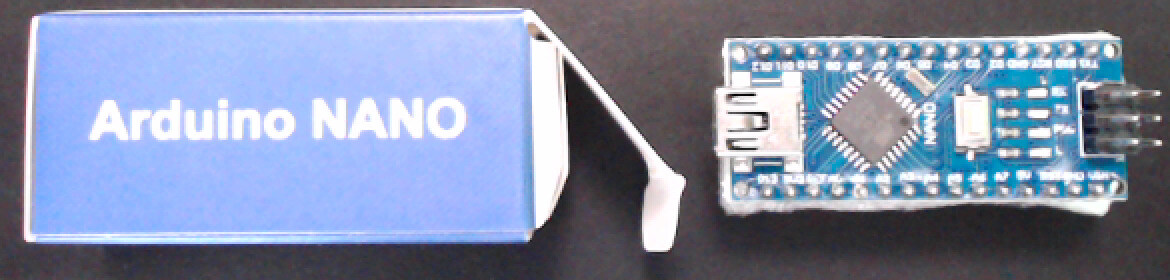
\includegraphics[height=2cm]{inventory/nano}}
    \renewcommand{\nandchipitem}{\item One (1) 74LS20\footnote{Any 74x20 or 54x20 integrated circuit is acceptable.} dual 4-input NAND integrated circuit \\ 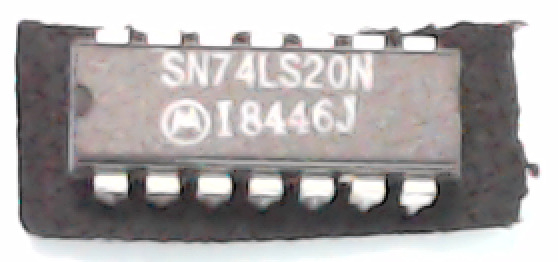
\includegraphics[height=2cm]{inventory/nand}}
}{}
\ifdefstring{\displaymodule}{MAX7219digits}{
    \renewcommand{\displaymoduleitem}{\item One (1) 8-digit 7-segment display module \\ 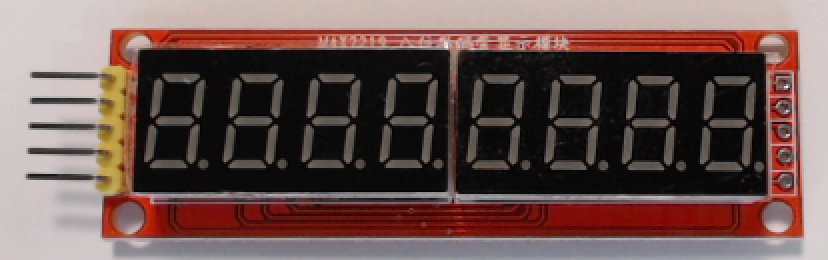
\includegraphics[height=2cm]{inventory/max7219digits}}
    \renewcommand{\fmcableitem}{\item One (1) 5-conductor 20cm ``rainbow'' cable (female-to-male) \\ 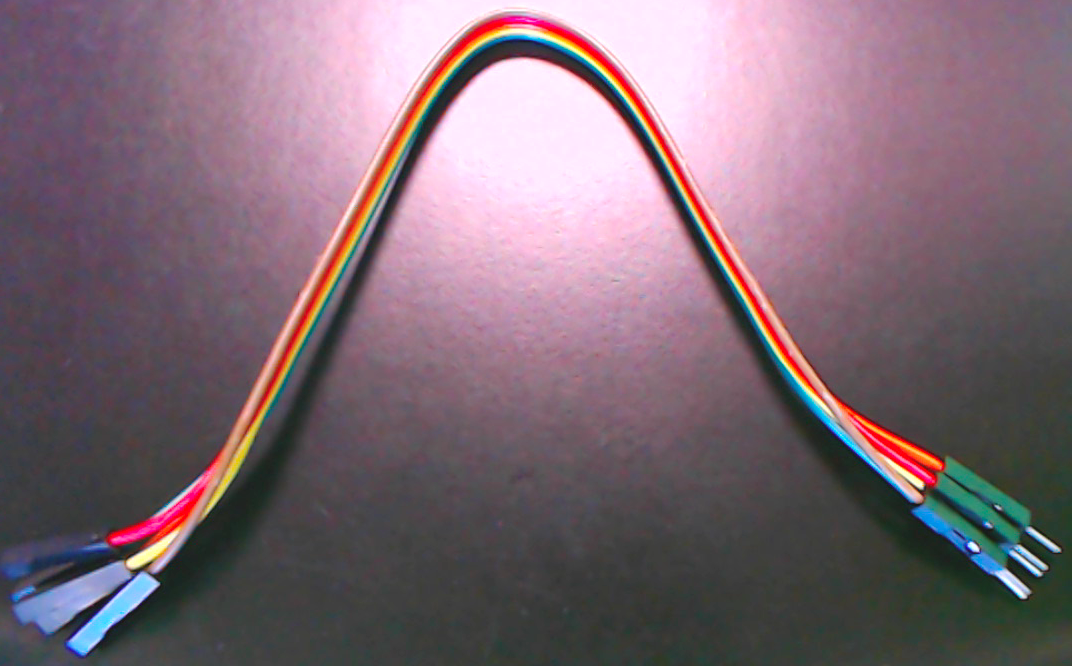
\includegraphics[height=2cm]{fm-5cable}}
}{}
\ifdefstring{\displaymodule}{MAX7219matrix}{
    \renewcommand{\displaymoduleitem}{\item One (1) $8 \times 8$ LED matrix display module \\ \textbf{\textit{Add LED matrix image here}}} %\includegraphics[height=2cm]{inventory/max7219matrix}}
}{}
%! suppress = MissingImport
\ifdefstring{\displaymodule}{LCD1602}{
    \renewcommand{\displaymoduleitem}{
        \item One (1) $2 \times 16$ character LCD display module \\ 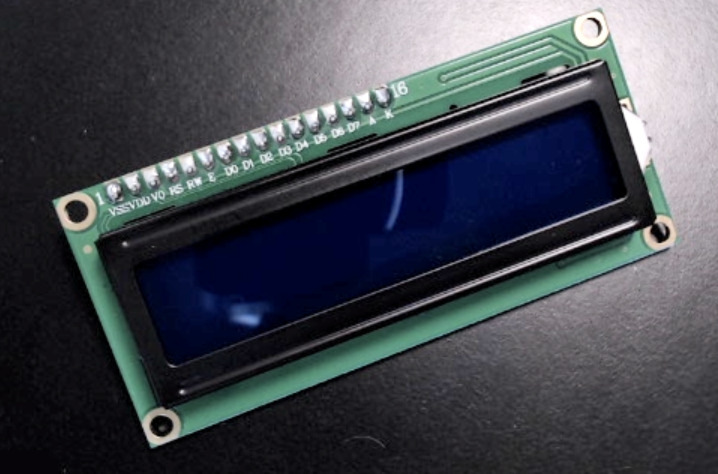
\includegraphics[height=2cm]{inventory/lcd1602}
        \ifdefstring{\serialprotocol}{I2C}{ \item One (1) I$^2$C-LCD Serial Interface (might be attached to display module) \\ 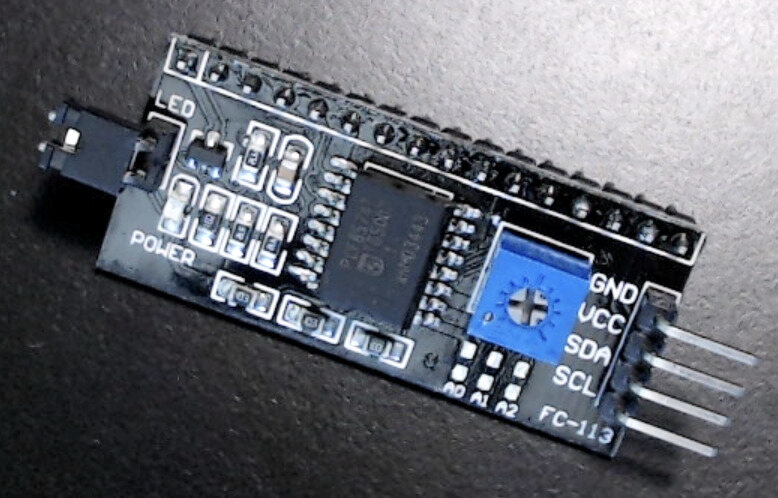
\includegraphics[height=2cm]{inventory/lcd-adapter} \hspace{1cm} or \hspace{1cm} 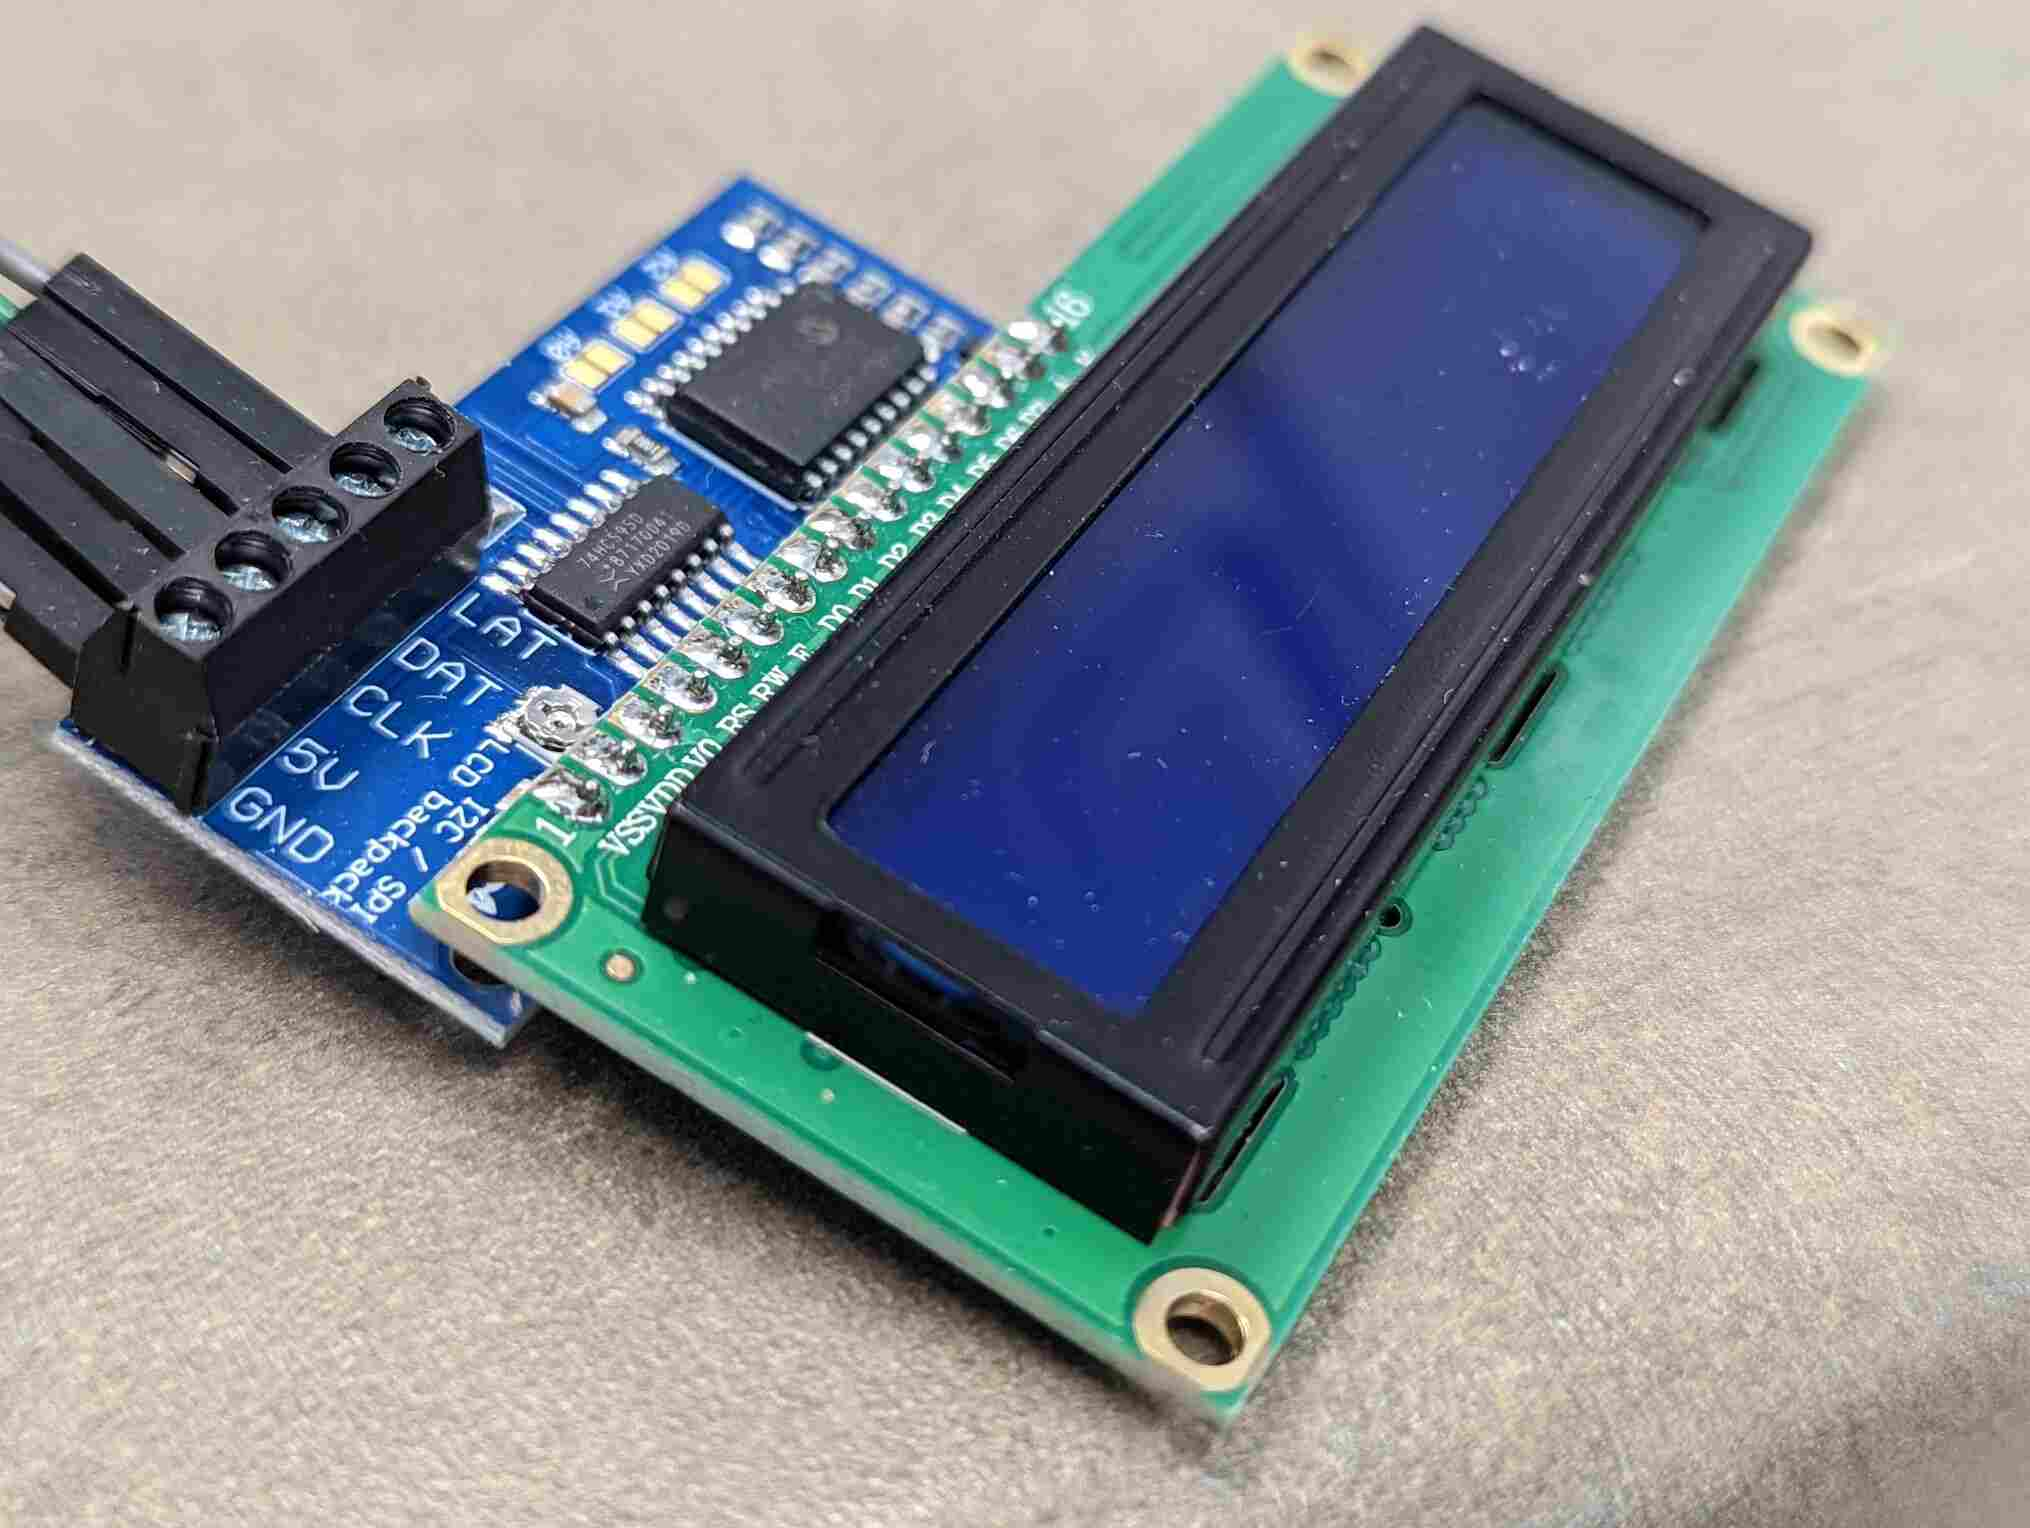
\includegraphics[height=2cm]{inventory/adafruit-lcd-adapter} \hspace{1cm} or \hspace{1cm} 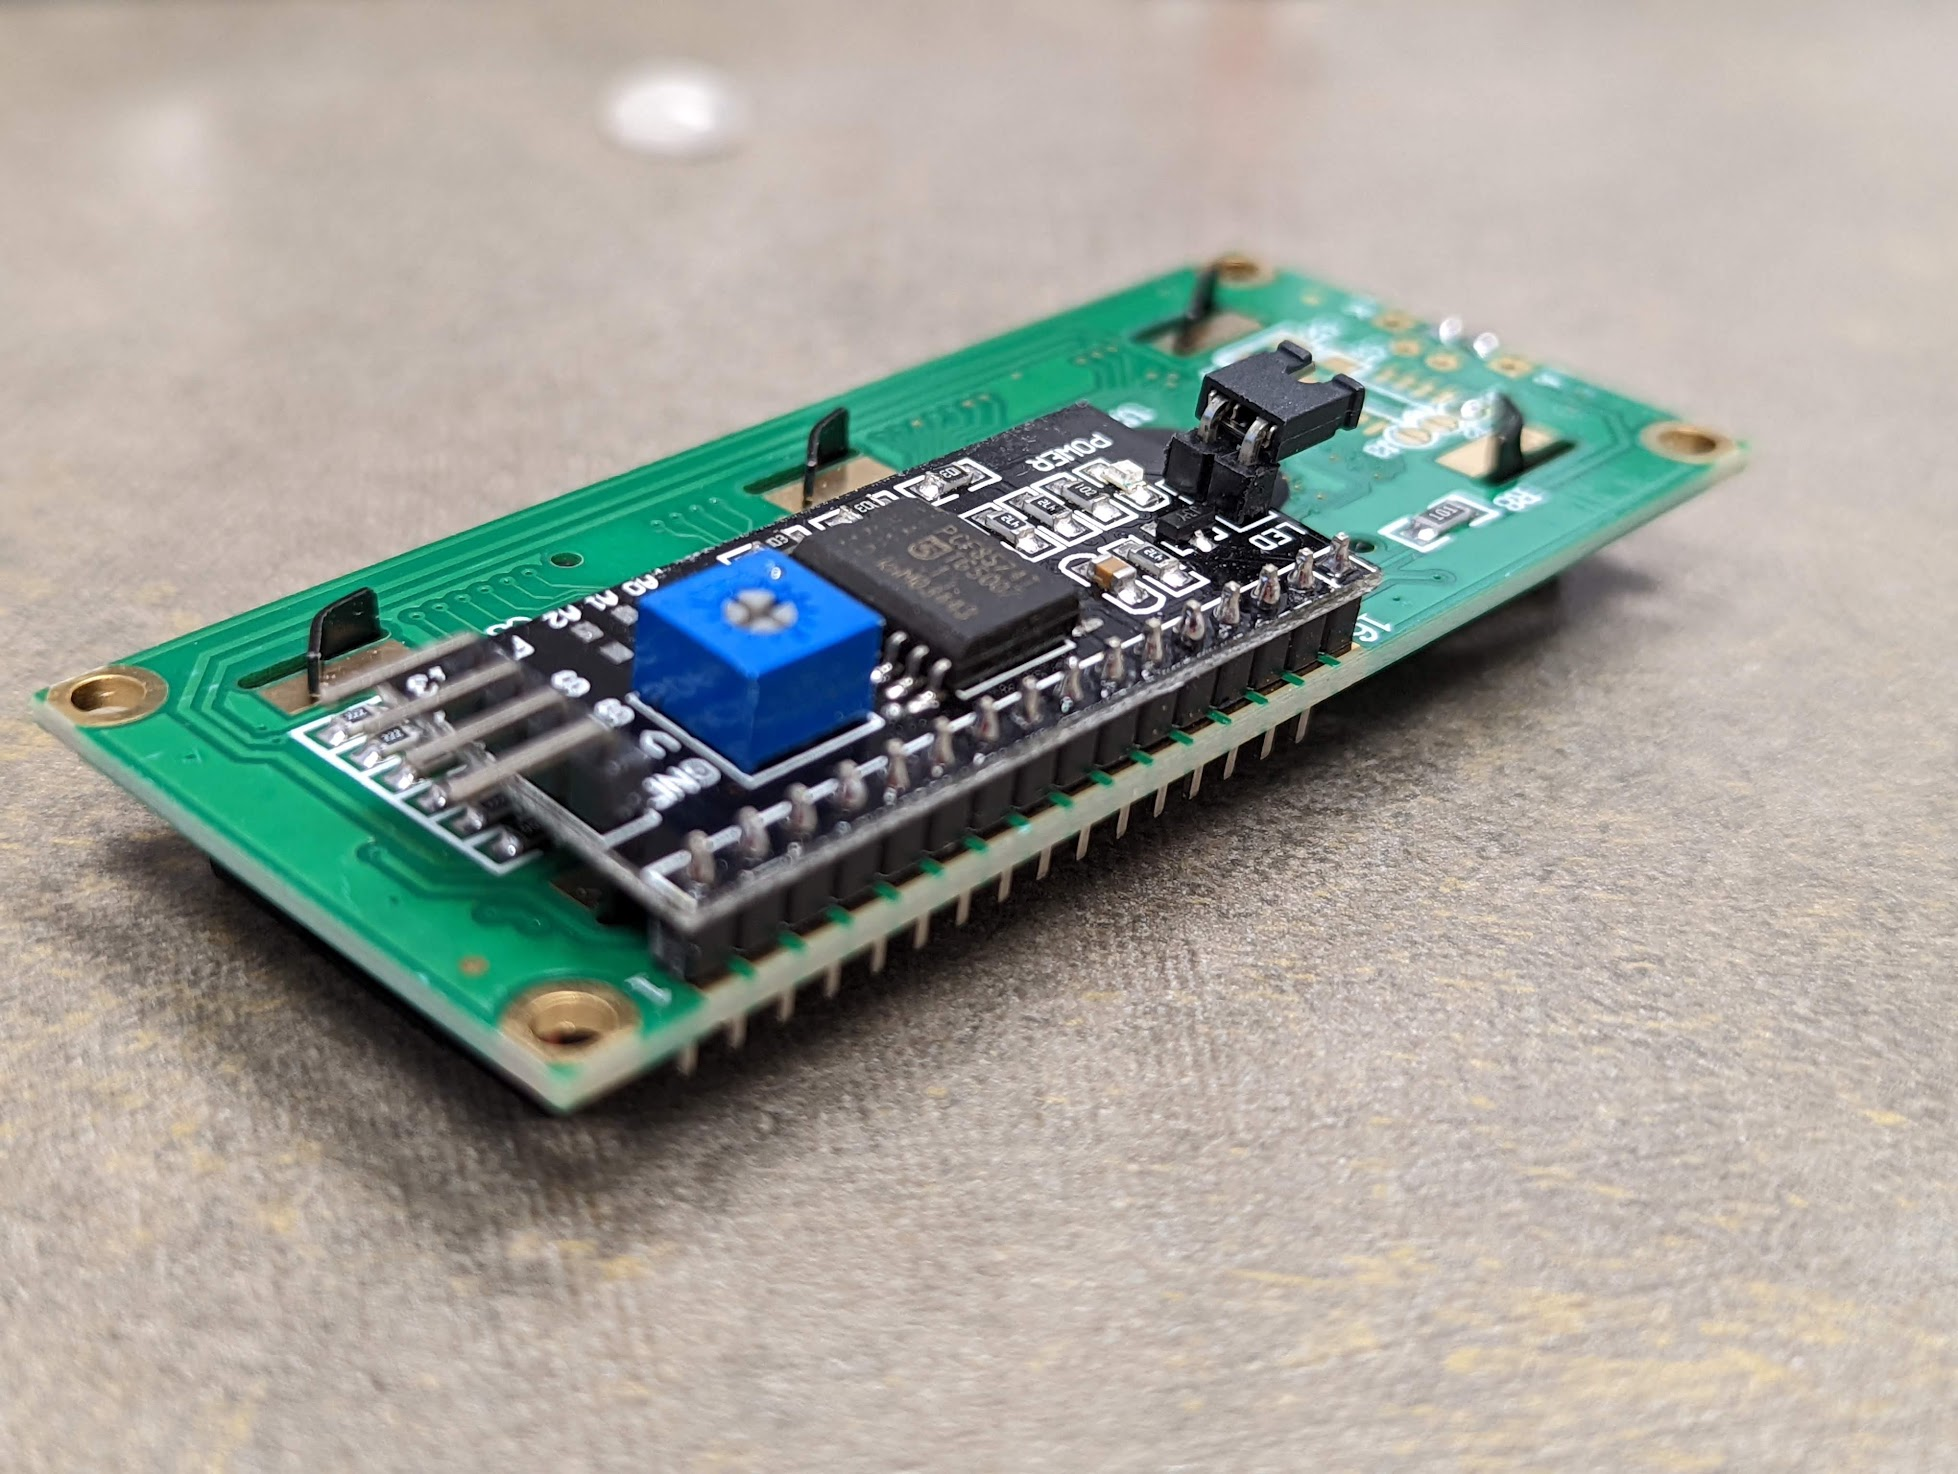
\includegraphics[height=2cm]{inventory/piggyback-lcd-adapter} }{}
        \ifdefstring{\serialprotocol}{SPI}{\item One (1) 74HC595 8-bit shift register \\ \textbf{\textit{Add shift register image here}}}{} %\includegraphics[height=2cm]{inventory/shiftregister}}{}
    }
    \ifdefstring{\serialprotocol}{I2C}{\renewcommand{\fmcableitem}{\item One (1) 4-conductor 20cm ``rainbow'' cable (female-to-male) \\ 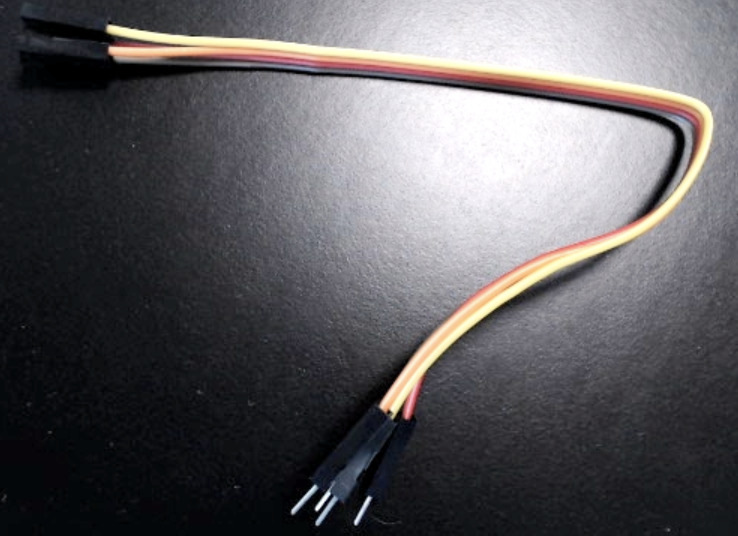
\includegraphics[height=2cm]{inventory/fm-4cable}}}{}
}{}

%%%%%%%%%%

Examine the contents of your class kit.
It contains:

%! suppress = MissingImport
\begin{itemize}
    \item One (1) full-sized solderless breadboard \\
        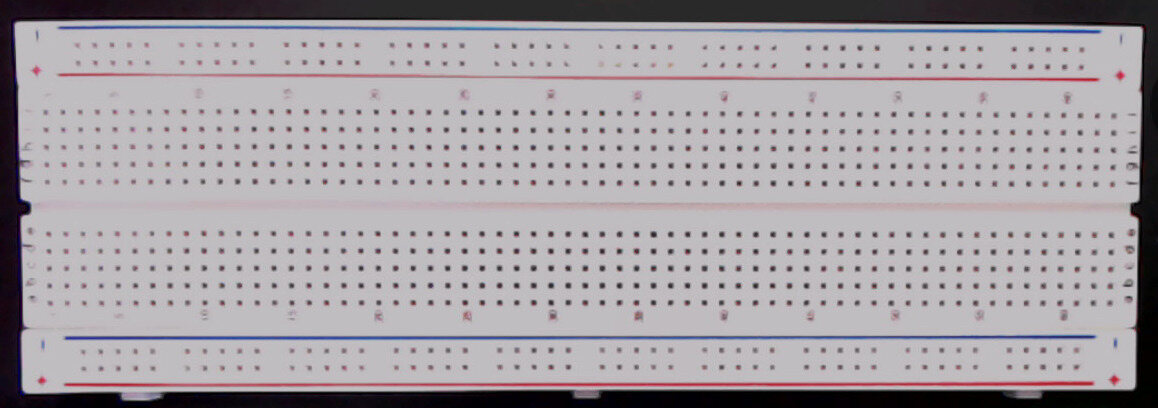
\includegraphics[height=2cm]{inventory/breadboard}
    \item One (1) \developmentboard\ (or clone) microcontroller board \\
        \devboardimage
    \item One (1) USB cable (mini-USB shown;
        yours may be different) \\
        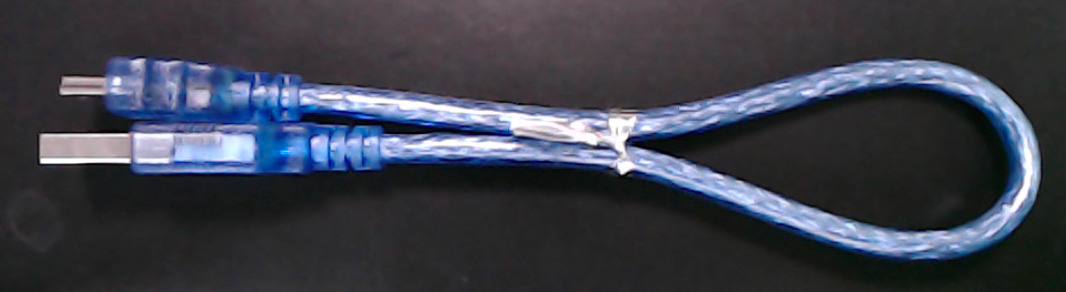
\includegraphics[height=2cm]{inventory/usb}
    \nandchipitem
    \item One (1) $4 \times 4$ matrix keypad \\
        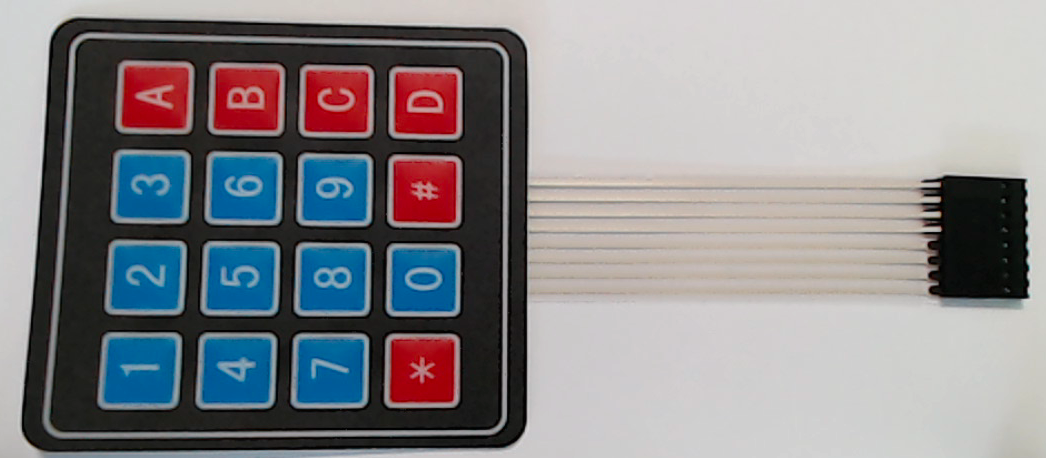
\includegraphics[height=2cm]{inventory/keypad}
    \item One (1) 8-pin male-male header strip (might already be inserted into keypad's female connectors;
        might have more than 8 pins) \\
        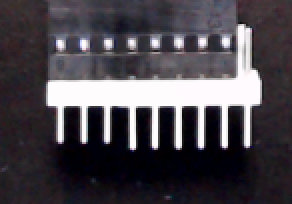
\includegraphics[height=2cm]{inventory/keypad-header-in-connector} \hspace{1cm} or
        \hspace{1cm} 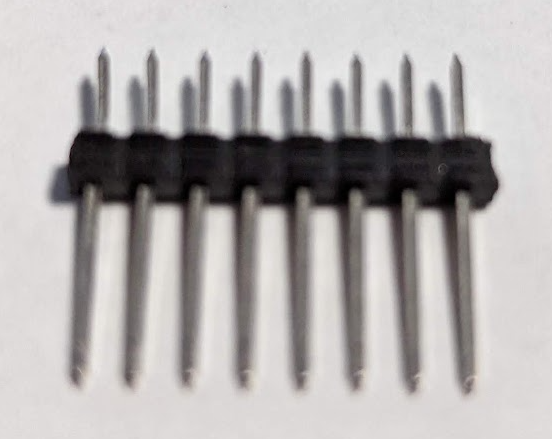
\includegraphics[height=2cm]{inventory/keypad-header-without-connector}
    \item Two (2) breadboard-mount momentary pushbuttons, aka tactile switches;
        these might have two leads (which might or might not be attached to cardboard strip), or they might have 4 prongs \\
        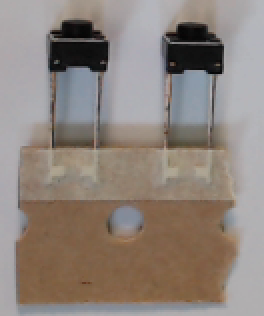
\includegraphics[height=2cm]{inventory/buttons-2pin} \hspace{1cm} or
        \hspace{1cm} 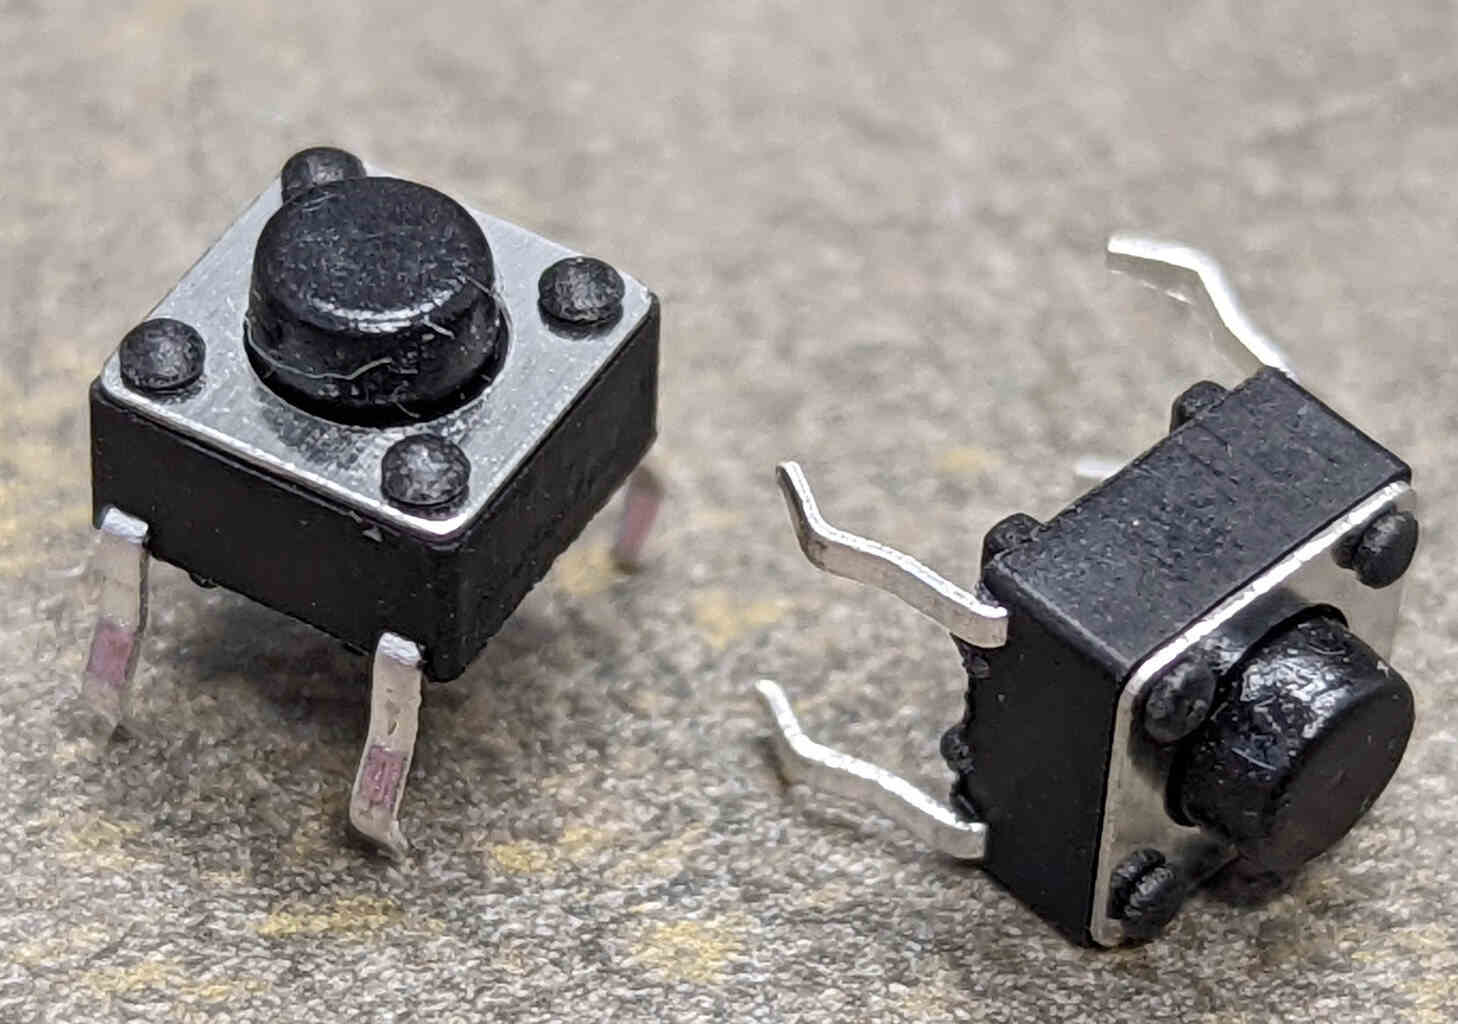
\includegraphics[height=2cm]{inventory/buttons-4pin}
    \item Two (2) breadboard-mount slide switches.
%    \item Two (2) breadboard-mount slide switches;
%        these might have three pins spaced 0.1in (2.54mm) apart, or they might have two pins spaced 0.3in (7.62mm) apart. \\
        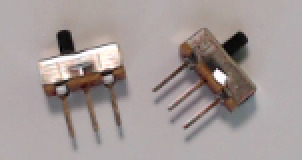
\includegraphics[height=2cm]{inventory/sliders-spdt}% \hspace{1cm} or
        %\hspace{1cm} \textbf{\textit{Add dip switch image here}} %\includegraphics[height=2cm]{inventory/sliders-dip1}
    \displaymoduleitem
    \item One (1) Light Emitting Diode (LED) (color may be different from shown) \\
        
\includegraphics[height=1cm]{inventory/led}
    \item One (1) 1k$\Omega$ resistor \\
        
\includegraphics[height=1cm]{inventory/resistor}
    \item One (1) 40-conductor 10cm ``rainbow'' cable (male-to-male), \textit{or} One (1) 20-conductor 10cm ``rainbow'' cable (male-to-male) and one (1) 20-conductor 20cm ``rainbow'' cable (male-to-male) \\
        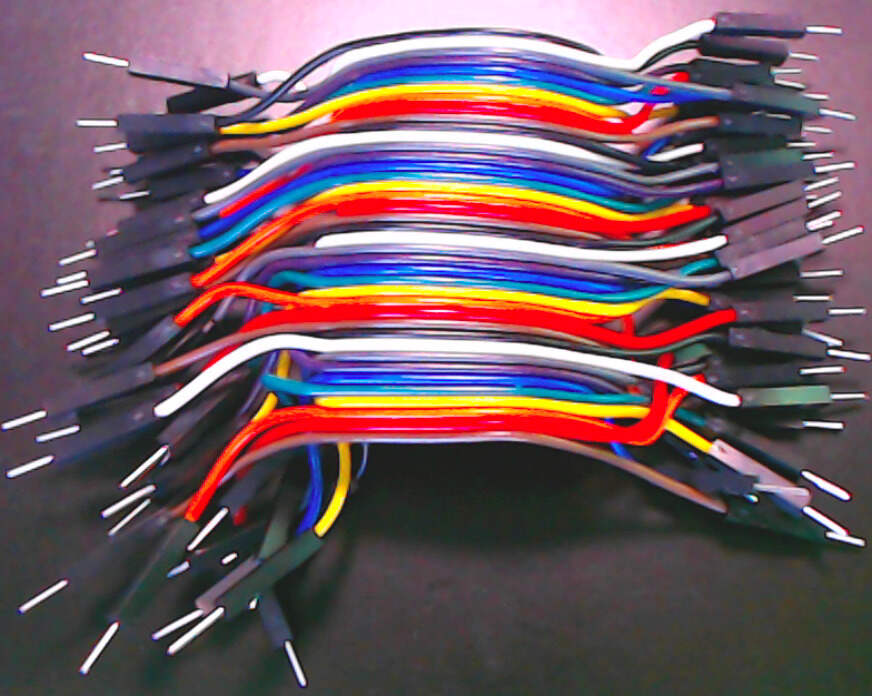
\includegraphics[height=2cm]{inventory/mm-cable}
    \fmcableitem
\end{itemize}

There may be other items in the class kit.
Set these aside;
you will not need them for this prelab, though they may be used in a specific lab.
